\documentclass[conference]{IEEEtran}
\pdfpagewidth=8.5in
\pdfpageheight=11in
%\usepackage{subfig}
\usepackage{subfigure}
\usepackage[pdftex]{}
\usepackage{graphicx}
%\usepackage{todonotes}
\usepackage{listings}
\usepackage{hyperref}
\usepackage{url}
\usepackage{todonotes}
\lstset {% general command to set parameter(s)
         language=C,
     basicstyle=\footnotesize,               % print whole listing small
%     keywordstyle=\color{black}\bfseries, % underlined bold black keywords
%     identifierstyle =\color{black},  % nothing happens
%     commentstyle=\color{black}\emph, % white comments
     %stringstyle=\ttfamily,          % typewriter type for strings
%     stringstyle=\color{black},       % typewriter type for strings
         tabsize=4,
         showtabs=false,
     showstringspaces=false}
%can't figure this one out for particles bandwidth
%\usepackage[caption,label]{subfig}

\newcommand{\DDT}{D\textsuperscript{2}T~}
\newcommand{\DDTns}{D\textsuperscript{2}T}
\newcommand{\subsubsubsection}{\noindent\textbf}
\newcommand*{\captionsource}[2]{%
  \caption[{#1}]{%
    #1%
    \\\hspace{\linewidth}%
    \textbf{Source:} #2%
  }%
}
%\addtolength{\parskip}{-0.08in}

% in order for balance columns to work, it has to be before begin document...
%\balancecolumns

\begin{document}

\title{SuperGlue: Standardizing Glue Components for HPC Workflows}

\author{
\IEEEauthorblockN{Jay Lofstead\IEEEauthorrefmark{1}, Alexis Champsaur\IEEEauthorrefmark{2}, Jai Dayal\IEEEauthorrefmark{2}, Matthew Wolf\IEEEauthorrefmark{2}, Greg Eisenhauer\IEEEauthorrefmark{2}}
\IEEEauthorblockA{\IEEEauthorrefmark{1}Sandia National Laboratories
\IEEEauthorrefmark{2}School of Computer Science, Georgia Institute of Technology}
}

\maketitle

\begin{abstract}

The challenge for constructing HPC workflows is not the simulation, the
analysis components, or the visualization tools. Usable, off the shelf tools to
suit most needs are available. Instead, the labor and complexity is connecting
these components together. Typically, an application scientist will write
``glue'' scripts that convert the output of one workflow phase to the input of
the next.  In nearly all cases, the output is written to disk after each
phase, read and written for the ``glue'' conversion, and then read for the next
phase. Even in online workflows, in which different components execute concurrently,
custom glue code usually has to be written.
This heavy lifting is one of the major stumbling blocks preventing
standardized workflow frameworks from broad, general adoption. Attempts to
streamline this process have not gained traction because of the necessity to
still build these glue components. In essence, the workflow engine offered only
a few, relatively small advantages over hand-coding the entire workflow.

SuperGlue rethinks the custom glue components in the context of online
workflows to offer reusable glue components that can bridge the type mismatches
between the output of one workflow component and the input of the next. By
performing a series of generic filter and selector operations in a typed environment, the
same glue is usable, without modification, to connect components of different
workflows with very different data types to achieve a plug-and-play workflow
construction environment with know performance characteristics.

\end{abstract}

%\category{D.4}{Software}{Operating Systems}
%\category{D.4.7}{Operating Systems}{Organization and Design}[hierarchical design]

%\terms{Design, Performance}

\section{Introduction}
\label{s:intro}

As extreme computing architectures continue to evolve, it is increasingly
clear that I/O is an increasingly significant problem.  Projections suggest no
significant parallel file system I/O bandwidth growth through the next 100x
increase in compute capabilities.  The traditional HPC approach of writing
complete checkpoints or analysis dumps for later processing to gain scientific
insights is becoming infeasible.  Even with technologies like Burst Buffers,
limited capacity reduces the usefulness. As such, in situ and in transit
analysis and visualization toolkits with the capability to reduce, process, and
otherwise mitigate the raw increase in data volume and throughput requirements
are increasingly important.

Existing workflow engines, such as Kepler~\cite{bertram:2006:kepler} and
DAGMan~\cite{Malewicz:2006:dagman}, offer flexible ways to assemble components
with rich functionality to manage the control flow. What they both lack is a
way to easily deploy and manage the glue code required to connect the various
components. One example illustrating the complexities comes from the Oak Ridge
Leadership Computing Facility (OLCF).  Kepler was used for several workflows
for the fusion simulation users.  While the initial goal was that an internal,
expert resource would create the workflow, including glue components, it should
be able to be maintained easily by the application scientists. Unfortunately,
the complexities of making and maintaining the glue components as the output
shifted and managing the deployment required the expert to be involved
regularly as the configuration evolved and scaled.  Falling back to Python
scripts managed by the application scientist proved easier and faster to
maintain. While this approach using the parallel file system to stage
intermediate data was sufficient, it is quickly becoming infeasible. The IO
overhead for using the parallel file system is exceeding acceptable runtime
percentages forcing a reduction in output and making scientific insights more
difficult to discover.

To address the performance mismatch, Integrated Application Workflows (IAWs)
are being developed. The easiest way to think of these IAWs is the Unix/Linux
shell pipe operator to connect commands. The shell connects stdout of one
program to stdin of the next with the assumption that each component in the
chain can operate in this mode. For tasks at this scale, this approach works
well. For the scientific workflows we are targeting, we have processes spread
across potentially 10,000s of nodes connected to other components also running
on multiple nodes. Unlike the command-line tools, none of these components
generally have the ability to shift their input or output from how it is
written to connect to a new online component without potentially significant
code changes. The challenge with these workflows is dealing with the lack of a
persistent store to stage intermediate data, interfaces for communicating data
state and availability, and data organization changes required before a
component can process data.  Each of these has been investigated by different
projects over the last several years.

Several frameworks have been developed that offer some functionality for
supporting online workflows. The more advanced examples incorporate some data
processing components, sometimes of limited scope, for performing in situ or in
transit processing. Data Staging~\cite{nisar:2008:staging} and in particular
data staging with processing
capabilities~\cite{abbasi:2009:datastaging,ober:seismic}, are a solid step
forward. The ADIOS IO library~\cite{lofstead:2009:adaptable} was designed with
this use case in mind. The HDF5 Virtual Object Layer
(VOL)~\cite{chaarawi:2013:hdf5-vol} was developed to support similar
functionality.

Several efforts to work through some of the issues related to IAWs have been
investigated~\cite{karimabadi:2013:catalyst,whitlock:2011:libsim,Glean,Flexpath,dreher:2016:bredala,zheng:2010:predata},
and much on-going research in the space promises to expand on some of the
needed techniques for management and placement.  Some
scientific codes have been addressing similar constraints for years by
in-lining analytics functions and performing complicated MPI communicator
subdivisions to allow simulation and analytics to co-exist.  One key
observation, however, is that there is a lack of portability to the resulting
implementations; they require a great deal of tuning and/or runtime placement
control to make them function as desired.

This paper describes our work on SuperGlue, a set of generic, reusable
components for composing scientific workflows. These are distributed data
analysis and manipulation tools that can be chained together to form a variety
of real-time workflows providing analytical results during the execution of the
primary scientific code.  Unlike existing components used in IAWs, SuperGlue
components do not have a fixed data type.  This one change enables using these
components on completely different kinds of simulations that share nothing in
their output format. Key to making this work is using a typed transport
mechanism between different components. Many options exist for these transports
and the particular mechanism selected is not critical. 

While the main contribution of this work is the design of generic \textit{glue
code}, the \textit{analytical} components we use in the workflows we present
here are designed using the same approach. For example, an index selection tool
is more of a glue component while a histogram component is more analytical.
Yet, we design both types of components as single MPI executables with similar
input and output interfaces launched using similar configuration options.  By
blurring the line between generic glue components and generic analytical
components, we present a flexible way to assemble scientific workflows without
having to write any additional code. 

The rest of the paper is organized as follows. First is a survey or related
work in Section~\ref{s:related}. Second, in Section~\ref{s:workflow}, is a
discussion of the two workflows we use to drive our insights. Next is an
overview of the concepts behind SuperGlue in~\ref{s:design}.  In
Section~\ref{s:reusable-components}, we provide an overview of the reusable
compoents created. In Section~\ref{s:integrating-reusable-components}, we
discuss the challenges of integrating reusable components.  An evaluation is
presented next in Section~\ref{s:eval}. Finally is a discussion of Conclusions
and Future Work in Section~\ref{s:conclusion}.

\section{Related Work}
\label{s:related}

Existing workflow systems have typically only been able to offer generic,
reusable components when the workflow system is for a particular niche with a
fixed datatype and standardized interfaces. For example, enterprise document
processing systems may all work against a single database with each user only
seeing their current worklist. As documents are processed, they are moved to
the next work queue, or completed state, according to hand-coded
rules~\cite{mckesson-workflow}. The Workflow Management Coalition~\cite{wfmc}
has developed standards to make enterprise process workflows more portable.
These standards are not intended to make components reusable, but to make
different workflow engines able to inter-operate or to port a workflow from one
engine to another.  The actual communication interfaces and data types are left
to the components themselves.

More directly related to this work and the scientific community are workflow
engines and frameworks custom made for the parallel computing environment.
Pegasus~\cite{mullender:pegasus} and DAGMan~\cite{Malewicz:2006:dagman} work
together to offer an engine to execute a workflow and a front-end system to
construct the workflow process itself. This pair does nothing to address the
actual connection between components. Instead, it is purely focused on
providing a usable system for assembling components into a scientific workflow.
This increment over a hand-crafted system should not be underestimated. It is a
significant amount of work to make this work well.

Kepler~\cite{bertram:2006:kepler} offers a nice GUI for assembling different
kinds of scientific workflows. It offers different directors to manage how the
workflow will be executed. Each component is an actor with channels connecting
actors. Some simple decision channels are available to offer different
execution paths given different output or return values from actors. As
mentioned in the Introduction, complex workflows using Kepler have been
assembled for many communities, including fusion science. Much like the Pegasus
and DAGman pair, Kepler focuses on offering starting components and managing
the control flow rather than offering standard interfaces and generic, reusable
components.

To address much of the complexity of communicating between separate parallel
components, in situ approaches are being investigated.
Catalyst~\cite{karimabadi:2013:catalyst} offers a way to integrate the
ParaView~\cite{Moreland:2008:paraview} analysis and visualization system
directly into the simulation executable. Catalyst strips out many features to
reduce the memory footprint and then requires explicit calls from the host
application into Catalyst routines with predictable data types on in-memory
data structures. While this can work for limited kinds of data processing, two
limitations can cause problems. First, in an internal Sandia project in 2012,
the CTH shock physics code used ParaView both in situ and also in transit. The
in situ integration saw the executable grow from 30 MB to 300 MB and the
scalability was strictly limited due to design flaws in ParaView for in situ
use. While this project prompted the creation of Catalyst, this stripped down
version of ParaView does not address all concerns. There is still a memory
footprint overhead and a runtime pause in the simulation progress for the
analysis and visualization to run.

Libsim~\cite{whitlock:2011:libsim} has a similar relationship to
VisIt~\cite{Riedel:2007:visit} as Catalyst has to ParaView. Both Libsim and
Catalyst have a strict limitation that offline workflows do not. In both cases,
because they are running on the same nodes as the simulation, time series
analysis and visualization can be difficult or impossible. The potential
scaling impact on the simulation because of limitations in Libsim or Catalyst
can prevent their use for the most important use cases at extreme scale.

A middle path between in situ and offline processing was investigated in
PreDatA~\cite{zheng:2010:predata}.
This work demonstrates that the placement of the analytics can significantly
affect the performance of workflows, and that this placement can be determined
in part by the communication characteristics of the analytics components.

Glean~\cite{vishwanath:2011:glean}, Nessie~\cite{oldfield:lwfs-data-movement},
and Mercury~\cite{Soumagne:2013:mercury} are intended to facilitate offering
portable workflows across different interconnect technologies. While their
origins may not have been directly for addressing workflows, they have been
re-purposed to address this field. Rather than offering anything related to
managing data types, these tools simply offer a portable way to construct
workflows.

A more active approach to managing workflow throughput was attempted in
FlexPath~\cite{Dayal:2014:flexpath}. Rather than focusing on the components
themselves, Flexpath offers mechanisms to monitor input queues for workflow
components and to redeploy components to reduce bottlenecks. It also has the
ability to redirect output from an online workflow to disk in the case of an
unrecoverable failure. Due to its ability to support data transport between
distributed executables regardless of their placement, and due to the simple I/O
interface provided by ADIOS~\cite{lofstead:2009:adaptable},
which supports FlexPath as one of its underlying
transport mechanisms, we use FlexPath and ADIOS in the workflows described
in this work.

Companion work to SuperGlue within this same project is
Bredala~\cite{dreher:2016:bredala}. This work presents an attempt to build a
data model for in situ workflows. It has some similarity to
FFS~\cite{eisenhauer:2011:ffs}. Unlike FFS, which is part of a much more
complex infrastructure for typed messaging between distributed processes,
Bredala is strictly focusing on the data model.

Overall, while all of these efforts are addressing different portions of the
online workflows puzzle, none of them are addressing the idea of general,
reusable glue and analytical components for scientific workflows.

\section{Workflows}
\label{s:workflow}

We designed and implemented two realistic real-time workflows based on
scientific codes having large user bases: the LAMMPS Newtonian particle
simulator~\cite{plimpton:1997:lammps} and GTCP, a particle-in-cell Tokamak
simulator~\cite{lin:gtc}. While both of these workflows eventually turn the
simulation data into histograms of certain quantities of interest, how they
arrive at their final result varies significantly. Creating similar types of
results, and this using some of the same components but in significantly
different ways, has allowed us to gain important insight into how best to
design glue components that can be used in a wide variety of workflows. We
first describe the workflows from a general point of view and then the
individual components in greater detail.

\subsection{LAMMPS Workflow}

We configure LAMMPS to simulate a disruption (a ``crack'') in a thin layer of
particles and outputs 5 numerical properties describing each particle in the
simulation at regular timestep intervals. This corresponds to two-dimensional
data (particles as one dimension and properties of interest as another) and
among these properties are the three-dimensional components of the particles'
velocities. In this case, the workflow outputs one histogram per timestep
showing the velocity distribution for all simulation particles at that point in
time.  From the LAMMPS output, the particular quantities of interest must be
extracted and then a histogram generated.

\subsection{GTCP Workflow}

\begin{figure}
\centering
\vspace{-0.10in}
  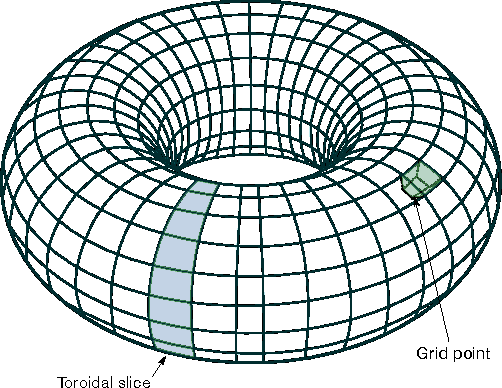
\includegraphics[width=0.7\columnwidth]{fig/Simple_Torus_mod}
\vspace{-0.15in}
  \caption{Representation of GTCP Toroid, modification of \cite{WikimediaCommons:torus}}
  \label{fig:toroid}
\vspace{-0.20in}
\end{figure}

GTCP, a code that simulates a toroidally confined plasma, splits the solid into
toroidal slices, each made up of a number of grid points. For each of these
grid points, it outputs 7 properties of the plasma such as pressure and energy
flux. This division of the toroid is illustrated in Figure~\ref{fig:toroid}.
The output of the simulation is therefore a three-dimensional array in which
the dimensions span: (a) toroidal ranks (toroidal slice number), (b) grid point
numbers, and (c) property indices. In this workflow, the per-timestep histogram
generated will show the parallel pressure distributions across
the entire simulation. From GTCP's output, the particular quantities of
interest must be extracted and then a histogram generated.

\subsection{Discussion}

In both cases, some particular quantity of interest is extracted from the
output data set, a calculation is performed, and a histogram is
generated. This is illustrated in Figure~\ref{fig:generic-workflow}. In many
cases, the histogram component may be some standard, reusable operator.
The challenge is the data selection and mathematical
manipulation to obtain the quantities of interest in a way that (a) presents an
intuitive interface to the scientist constructing the workflow and (b) is
useful in different types of workflows in which data have different sizes and
dimensions.  This difficulty arises because (a) the data at each stage of the
workflow is distributed over the collection of processes involved in each
component even if it forms a coherent whole and (b) the extraction and
re-arrangement of multi-dimensional, distributed data, in a way that is
configurable by the user at runtime is challenging.  Both workflows are
similar, insofar as both codes generate a large output while we are only
interested in a per-timestep histogram of a particular simulation quantity.
However, because the simulations generate very different data, selecting the
relevant data from the simulations and formatting it in a such a way that the
final Histogram component can operate on it is done very differently in each
workflow.

\begin{figure}[htbp]
\vspace{-0.10in}
\centering
\includegraphics[width=0.7\columnwidth]{fig/gwflow}
\vspace{-0.15in}
\caption{Generic Workflow Illustration}
\label{fig:generic-workflow}
\vspace{-0.25in}
\end{figure}

In typical scientific workflows today, custom glue code is written for
selecting relevant data and writing it so the ``formatter'' illustrated in
Figure~\ref{fig:generic-workflow} can work.  Then, potentially additional
custom glue code will fix the histogram calculation into something that can be
rendered or saved as desired.  In this work, we demonstrate general, reusable
components capable of handling all three intermediate operations.

The workflows presented here use no custom glue code. Instead, the glue is
designed as generic components that accept command-line configuration options
at launch time. At most, the user specifies a few parameters and organizes
the components into a proper pipeline. Both of these operations are easy enough
that a non-expert
%application scientist
can create workflows through GUIs or other guided assembly techniques.

That we are able to use some of the same glue code to connect the start to the
end of each workflow shows that generic glue code that can manipulate large
datasets in real time is possible and useful for assembling very different
workflows.  In addition, we later show that generic components, both glue and
analytical, have the advantage of possessing known performance characteristics,
which greatly facilitates the configuration of workflows that use them.

\section{Design}
\label{s:design}

In this work, we offer some insight in the design of generic data manipulation
and analysis components from our implementation of two workflows. These
workflows are driven by two different scientific codes, yet they share some of
the same components. First, we present our insights and then discuss our
implementation choices and how they affect the project.

\subsection{Key Insights}

By evaluating the presented workflows and considering other workflows with
which the authors are familiar, four particular insights are revealed.

\begin{enumerate}

\item To allow for the greatest variety of workflows, data manipulation
primitives and data analysis components should be packaged in similar ways —-
that is, regardless of their individual complexity, the pieces that make up
these workflows should export compatible interfaces as much as possible.

\item The ability to handle multi-dimensional data, along with the consistent
labeling of dimensions and quantities as meta-data, allows for components that
are highly adaptable and simple to use.

\item While different types of components understand varying levels of
semantics, maintaining a high level of semantics (i.e., labeling quantities and
dimensions as much as possible) early on and when passing through components
that do not necessarily require all of these labels allows for the most
functionality downstream.

\item Because programming languages understand multi-dimensional data as being
in a specific order in memory, there is a need for components that re-arrange
data and re-label its dimensions without necessarily changing its size. Indeed,
when data is contained in a database on disk, it is simple to gain a desired
view of the data, for example by using SQL. However, in the middle of a
real-time workflow, data must be presented to the components in a format that
they expect and understand. By allowing workflow components to support any
number of dimensions, by labeling these dimensions consistently, and by
developing components that re-arrange and re-label data, we can do this in a
generalizable fashion.

\end{enumerate}

These insights guide the design for the reusable components presented in this
paper. In particular, step decomposition for a workflow to enable more general
processing is preferred over more numerous, richer functionality components.

\subsubsection{Multi-Dimensional Data Support}

Many scientific codes serialize their output, effectively packing
multi-dimensional data into a single dimension. However, this technique offers
little information on the data to downstream components in a workflow. In the
case of our LAMMPS workflow, for example, if we kept the simulation output
one-dimensional, downstream components would have to be specifically designed
to read data in this format, and such components could not be easily made to
work with serialized data having other formats. In our example, a separate
component would have to be designed to work with the output of GTCP.

In order to use the same {\em Select} component downstream from both LAMMPS and
GTCP, we had to (a) modify the output of LAMMPS to let it output data in a
format where the dimensions are clearly defined, and (b) we had to design {\em
Select} in such a way that it understand input data having any number of
dimensions.  Indeed, even with the modification to LAMMPS, the simulation’s
output is two-dimensional, whereas the output of GTCP is three-dimensional.

In general, it is advantageous to (1) design components that can operate on
multi-dimensional data as much as possible, and (2) format the ouput data of
scientific applications as having well-defined dimensions. Emphasizing the
support for multi-dimensional data in the design of workflow components allows
for maximum compatibility between the interfaces of components by providing a
consistent way to refer to the data. With {\em Select} supporting any number of
dimensions, the user can simply indicate at runtime which dimension to select
from. Similarly, in {\em Dim-Reduce}, any dimension can ``absorb'' any other
dimension, as long as these dimensions are correctly specified by the user.
Such functionality increases the generic quality of these components and
simplifies their use. In our implementation, {\em Magnitude} expects
two-dimensional data, but allowing this component to support any number of
dimensions would be both feasible and advantageous.

Still, while multi-dimensional data support provides a consistent way to refer
to the data, not all components should be designed so as to work with
\textbf{\em any number} of dimensions. For example, we found it advantageous to
design {\em Histogram} to work with only one dimension. Creating a histogram is
a calculation that makes sense for one-dimensional data, and supporting a
higher number of dimensions would add unnecessary complexity this component. If
the data has more dimensions than are expected, or if only certain indices in
one dimension hold values of interest, we can use the {\em Dim-Reduce} and {\em
Select} components to properly format the data for {\em Histogram}, as we do in
the GTCP workflow.

\subsubsection{Semantics}

When data is organized under clearly defined dimensions, labeling these
dimensions as the data goes through each component lets downstream subscribers
refer to dimensions using their names. Because the data is potentially re-sized
and re-arranged in the course of a workflow, it is useful to maintain such
semantics as much as possible. However, the absence of labels should not block
the workflow execution. We did not label dimensions in the components and
workflows we implemented, rather refering to them by number, but this optional
functionality can be easily added and the advantage of doing so in the
development of more complex workflows is clear.

In both workflows, we do however label the \textbf{\em quantities} in one of
the dimensions so that the {\em Select} component can extract some of these
quantities using their names. These names are concatenated into a ``header
string'' using a well-known character as a separator. Because {\em Select} is
used as the first analytical component in both workflows, we are only concerned
with the existence of this header in the simulations and in the {\em Select}
components. We write this header in the output of the simulations and read it
when the data arrives at {\em Select}.  Using {\em Select} further downstream
poses a problem, however. In our current implementation, knowning which
quantities to select requires such a header, and ensuring the existence of this
header at any point downstream would require labeling all quantities at every
component, which would be highly impractical.  As a solution, we suggest
providing a choice to the user between using a header and using index numbers
to select quantities. Then, if the header exists, the quantities' names can be
used, and if {\em Select} needs to be used downstream and there is no header
describing the quantities, the user can provide the indices of the quantities
to select. We see here that labels should be used as much as possible, but that
they should also be kept {\em optional}.

\subsubsection{Dimension Recution (\em Dim-Reduce)}

In the context of scientific workflows, there are some situations where it is
desirable to eliminate one of the dimensions of a multi-dimensional array
without losing any of the values stored in the data set, and without changing
the meaning of some of the other dimensions. For example, in its output, GTCP
keeps track of the toroidal slice that produces the data of interest by using a
dimension that spans the ``Toroidal rank'' of grid points. In our workflow, we
wish to create histograms encompassing all grid points in the toroid, thereby
eliminating the concept of ``Toroidal rank'' and instead growing the dimension
that spans the number of grid points.

Programming languages represent multi-dimensional arrays in a specific order in
memory, so we cannot simply keep the data ordered as it is, change the number
of dimensions and their sizes, and assume that the new dimensions correctly
reference the data. In fact, here we demonstrate that even though {\em
Dim-Reduce} does not modify the size of the data, it potentially requires a
rearrangement of the data in memory, so that the data is correctly represented
by the new dimensions. We also show that a simple calculation can be used to
obtain new indices in the dimension that grows.

\subsubsubsection{Dim-Reduce: Description}

Because the motivation for this operation is based on how people understand
data, rather than how it is represented internally, it is best explained
through an example. Say that we have a solid divided into 6 sections. In each
section, there are 3 particles for each of 4 charge types and 2 colors. We have
a 4-dimensional array holding the speeds of all particles, for each value of
these attributes (section, particle number, charge type, color). The dimensions
of the array are $N_0{\times}N_1{\times}N_2{\times}N_3$, where:

\begin{itemize}

\item $N_0 = 6$ is the size of the {\em section} dimension $D_0$

\item $N_1 = 3$ is the size of the {\em particle number} dimension $D_1$

\item $N_2 = 4$ is the size of the {\em charge type} dimension $D_2$

\item $N_3 = 2$ is the size of the {\em color} dimension $D_3$

\end{itemize}

Now, say that for the purpose of performing some type of analysis on the
dataset, we wish to eliminate the concept of {\em color} of a particle and
compensate by changing the concept of {\em particle number}, so that $D_1$
spans all particles in a particular section and of a particular charge type,
regardless of color. We still wish, however, to keep track of the original
section where the particle is located and of its original charge type. The
desired result of this operation is that:

\begin{itemize}

\item The concept of {\em color} of a particle disappears

\item The concept of {\em particle number} loses its original meaning and takes
on a new one. Its dimension now spans all particles in a particular section and
of a particular charge type, regardless of color.

\item The concepts of {\em section} and {\em charge} keep their original
meanings, and the sizes of their dimensions are unchanged.

\end{itemize}

We can say that $D_1$, the {\em particle number} dimension, \textbf{\em
absorbs} $D_3$, the {\em color} dimension. The array resulting from this
operation has dimensions $N_0'{\times}N_1'{\times}N_2'$ , where:

\begin{itemize}

\item $N_0' = 6$ is the size of the {\em section} dimenson $D_0'$

\item $N_1' = N_1{\times}N_3 = 6$ is the new size of the {\em particle number} dimension $D_1'$

\item $N_2' = 4$ is the size of the {\em charge} dimension $D_2'$

\end{itemize}

We call this operation {\em dimension reduction}. Even though it does not
change the size of the data set, we can show that it potentially changes the
ordering of data in memory.

\subsubsubsection{Dim-Reduce: Data Re-Ordering}

In the original array, say we are interested in the speeds of the particles in
section number 3, and having charge type 1. This corresponds to all of the
particles with indices $(3, p, 1, c)$, where $p$ is any particle number and $c$
is any charge type. Assuming row-major order, the one-dimensional indices of
these quantities of interest are:

\begin{itemize}

\item 1-D indices of $(3, p, 1, c)$: 74, 75, 82, 83, 90 ,91.

\end{itemize}

After the dim-reduce operation described above, even though the concepts of
particle number and color have changed, we would like the indices in the
dimensions $D_0'$ and $D_2'$ to keep their original meanings. The operation
leaves us with a $6{\times}6{\times}4$ array, in which the 1-D indices of the
quantities of interest, that is, the speeds of the particles of charge type 1
in section number 3, are:

\begin{itemize}

\item 1-D indices of $(3, p' , 1)$: 73, 77, 81, 85, 89, 93.

\end{itemize}

In this case, we see that the one-dimensional indices of the same values before
and after the dim-reduce operation all differ. Therefore, in order to satisfy
the desired qualities of the dim-reduce operation, we potentially have to
re-order the data in its one-dimensional representation.

\subsubsubsection{Dim-Reduce: Calculation}

Using the same example, say $(s, p, ch, cl)$ are the indices of a value in the
original array, and $(s', p', ch')$ are the indices of the same value in the
new array (after the {\em dim-reduce} operation).

Because the new dimension $D_1'$ holds the new meaning for the particles, we
have some freedom in hat its indices represent, as long as they range from 0 to
$N_1{\times}N_3$ in increments of 1.

If we define the dim-reduce operation as:

\begin{itemize}

\item $s' = s$

\item $p' = p + (cl{\times}N_1)$

\item $ch' = ch$,

\end{itemize}

then the above requirements are met. This is simple to generalize to any number
of dimensions.

\subsubsubsection{Dim-Reduce: Conclusions}

\begin{itemize}

\item One dimension is eliminated, another dimension takes on a new meaning, and all other dimensions keep their original meanings.

\item This is useful in scientific workflows.

\item It potentially requires a re-ordering of data in its 1-D representation.

\item We can use a simple arithmetic operation to create new indices in the
dimension that grows.

\end{itemize}

\subsection{Implementation Artifacts}

While particular decisions are made to investigate the potential for reusable
components, the choices made are by no means the only tools and techniques for
achieving success. Rather, the selected technologies offer many features that
ease the creation of reusable components. The reasoning for these selections is
explored below.

Even though we refer to the components as single entities, they are distributed
codes that know how to split computation among the processes of which they are
composed. Since we need some analogy to the Linux shell pipe operator for
connecting components, we choose to use ADIOS for the flexibility in writing
destinations, reading sources, and offering a typed data stream. In particular,
we use the Flexpath transport. It implements a stream-based data exchange
abstracted to the components through the ADIOS interface, is asynchronous, and
allows for data exchange between any number of writers and readers. Therefore:

1. We can launch components of the workflow in any order: downstream components
will wait for the availability of data from upstream components, and upstream
components will buffer data up to a certain size until they are able to send it
downstream. This also means that the decision as to which downstream
components to use can be made after the upstream components have started
running, allowing for real-time adjustments to the workflow based on results
obtained upstream.

2. Even if the number of processes used for one component is different from that
used for the previous one in the workflow, each component can split the data
(and therefore the computation) evenly among its processes. We should mention,
however, that due to the current implementation of Flexpath there is overhead
data exchanged when different numbers of writers and readers are used. Even if
reader R requests only a portion of writer W’s data, the current implementation
is such that W sends all of its data to R. This is in the process of being
corrected and is orthogonal to the work done for this project.

In addition, ADIOS and its transports, such as Flexpath, keep track of the
data dimensions and their sizes. Therefore, when a component receives a
multi-dimensional array, it can discover the dimensions of the data and their
sizes as defined by the previous component in the workflow. Note that the
data type as input to one component may be changed for the output. This is
crucial for operators that select a data subset or generate a derived product.

When using a component, one must specify the names of the input stream from
which to read, the array in the input stream, the output stream to which to
write, and the name of the array to use in the output stream. Referring to
streams and arrays using names allows users to easily chain together these
components into potentially complex workflows. Certain components require more
information from the user. For example, Select must know from which dimension
to select the quantities of interest.

\section{Reusable Components}
\label{s:reusable-components}

\begin{figure*}
\vspace{-0.10in}
  \includegraphics[width=\linewidth]{fig/wflow3}
\vspace{-0.35in}
  \caption{LAMMPS Workflow}
  \label{fig:lammps-workflow}
\vspace{-0.10in}
\end{figure*}

\begin{figure*}
%\vspace{-0.10in}
  \includegraphics[width=\linewidth]{fig/wflow4}
\vspace{-0.25in}
  \caption{GTCP Workflow}
  \label{fig:gtcp-workflow}
\vspace{-0.30in}
\end{figure*}

After evaluating the example workflows selected the following components are
created to demonstrate the potential for reusable components.

\subsection{Select}

Given an input stream that includes an array with any number of dimensions,
Select extracts certain indices from one of the dimensions and outputs an array
with the same number of dimensions, but with the dimension of interest having a
smaller size. The output data of this operator therefore has a smaller overall
size than its input data. In order to select the quantities of interest, the
component uses a header which must be passed by the previous component in the
workflow. The header is a list of strings that name the quantities in the
dimension of interest. This allows easy selection of quantities at runtime when
Select is launched. For example, in the LAMMPS workflow, the simulation outputs
the ID, Type, Vx, Vy, and Vz of each particle, where Vx, Vy, and Vz are the
components of the velocity of the particle. Select discards the ID and Type of
the particle, building a new array consisting only of the velocity components
of each particle. The user, or a higher-level dataflow assembler, must pass to
this component the index of the dimension from which to select.

\subsection{Dim-Reduce}

As discussed previously, workflow components must receive data in a format
that they expect. For example, Histogram expects one-dimensional data.
Dim-Reduce is a data manipulation component that removes one dimension from its
input array, ``absorbing'' it into another dimension without modifying the
total size of the data. The other dimensions are left unchanged. This component
can work with an input array having any number of dimensions. The output is an
array with one dimension removed and with another dimension that has been
re-defined. We discuss this operator and the need for it in more detail in
Section~\ref{s:abc}. When using this component, the user must specify which
dimension to eliminate and which to grow.

\subsection{Magnitude}

In our current implementation, magnitude expects a two-dimensional array as
input, where one dimension spans the data points at each time step (particles
in the case of LAMMPS and grid points in the case of GTC), and the other
dimension spans any number of components of the same quantity, for example the
three-dimensional components of velocity in the LAMMPS workflow. Magnitude
calculates the magnitudes of these quantities from their components and outputs
a one-dimensional array of new values. Which dimension is which in the input
array is specified by the user at runtime. A small number of changes and a few
start-up parameters could generalize this code to work for many more cases.

\subsection{Histogram}

The processes that make up the Histogram component partition among themselves
a one-dimensional array of data. They communicate to discover the global
minimum and maximum values in the array, create a number of bins between these
two extremes, and then communicate again to count the number of values in the
globally partitioned array that fall in each bin. The number of bins to use
must be passed to the component when it is launched.

In our current implementation, one of the processes of Histogram writes the
output to a file on disk. We chose this approach because this component is
generally used as an endpoint in the workflow and because the output of this
component is generally small and can be easily written by a single process.
However, as we discuss later, letting this component output its data in the
same way as the other components, as an ADIOS stream, and instead writing to
disk when needed using a component specifically designed for this purpose would
provide greater flexibility.

\subsection{Dumper}

While this component was not created in time for this paper, the value
proposition is clear. As mentioned in the Histogram description above, this is
the component determined to be of value once the experiments were completed.
The key goal for this component is to offer a way to write a stream into an
output file using some particular format. Having a way to write HDF5, ADIOS-BP,
or a simple text file would all be simple variations.

Related to the realization of the value of separating out this functionality is
a desire to offer a graph plotting capability. Something like GNU
Plot~\cite{racine:2006:gnuplot} take a simple text input description and
generates a graph.  Incorporating such functionality into a component would
also be valuable.  Further, rather than having the graphing component write to
disk, it should also push out an ADIOS stream to some other consumer. An
additional Dumper that writes an image file in a particular format, such as
JPEG, PNG, or SVG, would be a valuable addition.

\section{Integrating Reusable Components}
\label{s:integrating-reusable-components}



In order to use some of the same components in both workflows, we had to
slightly modify the output stages of the scientific codes driving them. Because
in both workflows, the first component to receive the simulation data is
Select, each simulation has to write a header of its quantities in the
dimension to be selected from. Also, normally LAMMPS packs its two-dimensional
output into a single array. We modified this so as to let it write a
two-dimensional array, which better describes the output data and allows
downstream components to better understand it. Both simulations had to be
modified to enable the use of ADIOS for output. While the ADIOS integration was
not difficult, it was the hardest, most significant changes made to the
simulations. If the simulations already had ADIOS integrated, the changes would
be very minor ``de-optimizing'' output. In many cases, output loses most, if
not all, of its structure for either performance or ease of integrating with
analysis or visualization components. Since SuperGlue components can maintain
that additional structure and metadata to the benefit of downstream consumers,
removing the structure elimination code is more removing customizations for
particular data consumers rather than introducing code particular to these
components. It is arguable that it is also customization, but the modification
impact on the data is far smaller than other integrations.

\subsection{Demonstrating in the Workflows}

We reconstructed the LAMMPS to velocity histogram generation workflow using the
SuperGlue components and generated a workflow illustrated in
Figure~\ref{fig:lammps-workflow}. We annotate the figure with details about how
the data is manipulated at each step.


Data arrives from LAMMPS at the first component we designed, Select, which
extracts these velocity components from the data output by the simulation. From
Select, data is sent to Magnitude, another of our components, which computes
the magnitudes of the velocities. In our current implementation, Magnitude
outputs one-dimensional data, an array of the magnitudes it calculates, to the
final component, Histogram, which expects one-dimensional data as input. The
end result of this workflow is a series of histograms of the total velocities
of the particles. There is one histogram created at each timestep at which the
simulation would normally dump its data to disk.


The GTC workflow after reconstruction is illustrated in
Figure~\ref{fig:gtcp-workflow}. As with the LAMMPS workflow, this is annotated
with details about data for each step. Also note that while there are shared
components, the workflow is a little different.

In our workflow, data first arrives at an instance of Select, which extracts
one quantity of interest out of the 7. This quantity is the ``perpendicular
pressure,'' or pressure of the plasma perpendicular to the flow in the grid
point of interest. Even if it contains only perpendicular pressures, the output
of Select is still three-dimensional since this component maintains the
original dimensions of its input. Because the Histogram component expects
one-dimensional input, we first send the output of Select through two instances
of our Dim-Reduce component, each of which eliminates a single dimension of the
array without changing its total size. The final component, Histogram, outputs
a histogram of the perpendicular pressures of all grid points at each timestep
at which the simulation would normally output its data to disk.

\section{Evaluation}
\label{s:eval}

The evaluation is performed on Titan, the Cray XK7 machine at Oak Ridge
National Laboratory. It consists of 18,688 nodes each with 1 16-core AMD
Opteron CPU and 32 GB of RAM. The interconnect is a Gemini network. There is an
attached Nvidia Kepler K20X GPU with an additional 6 GB of memory on every
node.

%The evaluation is performed on Rhea, a capacity cluster at Oak Ridge National
%Laboratory. It consists of 512 nodes each with two 8-core 2.0 GHz Intel Xeon
%processors with Hyper-Threading and 128 GB of RAM. The interconnect is FDR
%Infiniband. For storage, Rhea uses OLCF's 32 PB Atlas Lustre parallel file
%system.

\subsection{Strong Scaling Experiments}

\begin{table*}[tbp]
%\vspace{-0.15in}
\centering
\caption{LAMMPS Evaluation Configuration Settings}
\label{tab:eval-strong-lammps}
\vspace{-0.15in}
\begin{tabular}{|l|l|l|l|l|}
\hline
Component Test & LAMMPS Procs & Select Procs & Magnitude Procs & Histogram Procs \\
\hline
Select & 256 & $x$ & 16 & 8\\
\hline
Magnitude & 256 & 60 & $x$ & 8\\
\hline
Histogram & 256 & 32 & 16 & $x$\\
\hline
\end{tabular}
\vspace{-0.15in}
\end{table*}

%LAMMPS setups:
%Select is 256:x:16:8
%Magnitude is 256:60:x:8
%Histogram is 256:32:16:x

\begin{table*}[tbp]
\centering
\caption{GTCP Evaluation Configuration Settings}
\label{tab:eval-strong-gtcp}
\vspace{-0.15in}
\begin{tabular}{|l|l|l|l|l|l|}
\hline
Component Test & GTCP Procs & Select Procs & Dim-Reduce 1 & Dim-Reduce 2 & Histogram Procs \\
\hline
Select & 64 & $x$ & 4 & 4 & 4\\
\hline
Dim-Reduce 1 & 128 & 32 & $x$ & 16 & 16\\
\hline
Dim-Reduce 2 & 128 & 32 & 16 & $x$ & 16\\
\hline
Histogram & 128 & 34 & 24 & 24 & $x$\\
\hline
\end{tabular}
%\vspace{-0.15in}
\end{table*}

%GTCP setups:
%Select is 64:x:4:4:4
%Dim-Reduce1 is 128:32:x:16:16
%Dim-Reduce2 is 128:32:16:x:16
%Histogram is 128:34:24:24:x

To obtain the results illustrated in
Figure~\ref{fig:lammps-strong},~\ref{fig:gtcp-strong-select},
and~\ref{fig:gtcp-strong}, we varied the process size of a single component at
a time while fixing that of the other components involved in the workflow.  We
determined reasonable process sizes for the fixed-size components using
preliminary testing. For all of these measurements, we set up the scientific
code driving the workflow to output a fixed total data size. Each point shows
the completion time for a single time step arbitrarily chosen in the middle of
the execution of the workflow. Depicted below the strong scaling curves are the
data transfer times. That is, these points show the portion of the timestep
completion time spent by the components waiting to receive requested data.

To understand the strong scaling behavior exhibited by the components in
different scenarios, we carried out strong scaling measurements of the
components in both the LAMMPS and GTCP workflows. The results for the LAMMPS
workflow are shown in Figure~\ref{fig:lammps-strong}, and those for the GTCP
workflow are shown in Figures~\ref{fig:gtcp-strong-select}
and~\ref{fig:gtcp-strong}. In all of the resulting curves, an informative point
is that at which the linear domain of scalability clearly ends. With process
sizes greater than those at these points, the benefit of adding more processes
for a fixed overall input size dwindles, and in most cases eventually reverses
due to communication overhead. Of course, no point on these lines is ideal for
all situations. For example, a scientist having few resources but significant
time at her disposal may wish to stay in the linear domain. However, these
turning points are a good single indicators of the strong scaling behavior of
our distributed components.

For Figure~\ref{fig:lammps-strong}, LAMMPS is run using 256 processes.  For
Figures~\ref{fig:gtcp-strong-select} and~\ref{fig:gtcp-strong}, GTCP is run
using either 64 or 128 processes. The actual process counts and the variable
factor for the LAMMPS workflow is listed in Table~\ref{tab:eval-strong-lammps}.
The GTCP workflow configurations are listed in
Table~\ref{tab:eval-strong-gtcp}.  The different factors are used to better
illustrate the overheads involved.

For the LAMMPS workflow, we present two different performance measurements to
better reveal the overheads involved. In these cases, we show both the amount
of time spent performing the data reads as well as the total time, including
the reading, for the component to operate.

\begin{figure*}[t!]
\vspace{-0.10in}
\center
\subfigure[Select]{
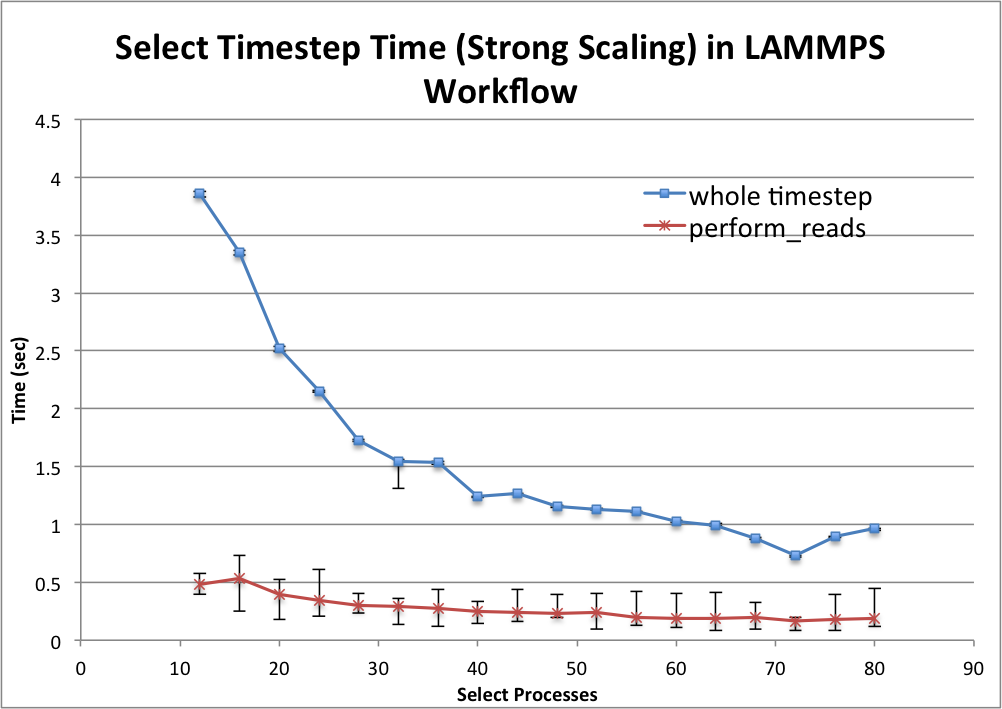
\includegraphics[width=0.3\textwidth]{fig/Titan-LAMMPS-Strong-Select}
\label{fig:lammps-strong-select}
}
\subfigure[Magnitude]{
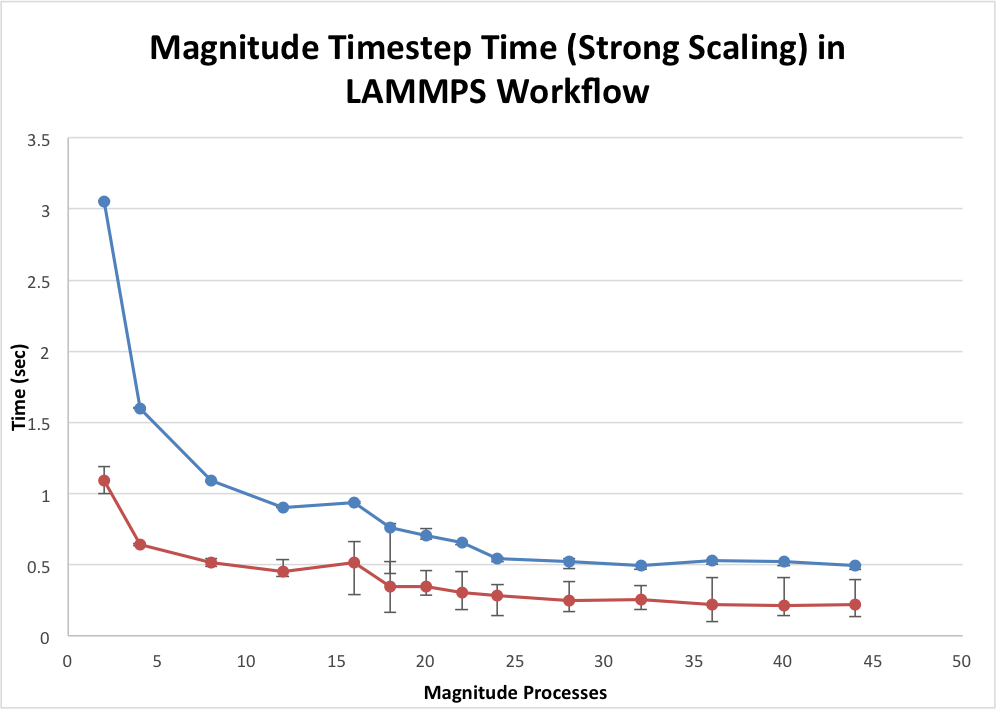
\includegraphics[width=0.3\textwidth]{fig/Titan-LAMMPS-Strong-Magnitude}
\label{fig:lammps-strong-magnitude}
}
\subfigure[Histogram]{
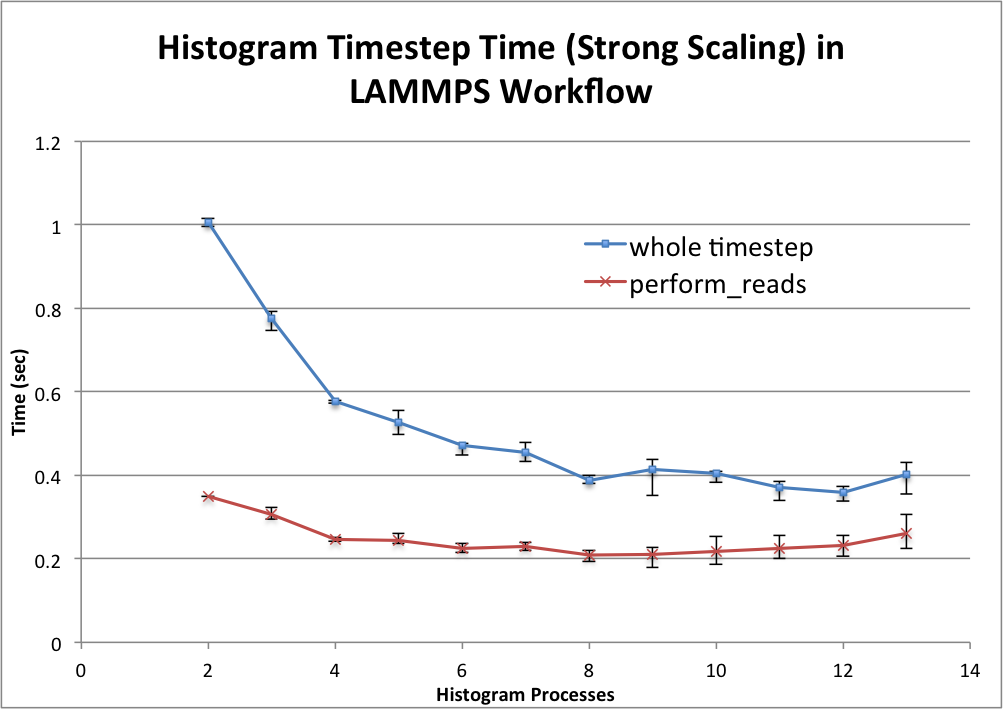
\includegraphics[width=0.3\textwidth]{fig/Titan-LAMMPS-Strong-Histogram}
\label{fig:lammps-strong-histogram}
}
\vspace{-0.10in}
\caption{SuperGlue Components Strong Scaling For LAMMPS}
\label{fig:lammps-strong}
\vspace{-0.10in}
\end{figure*}

\begin{figure*}[t!]
\vspace{-0.10in}
\center
\subfigure[Select-1]{
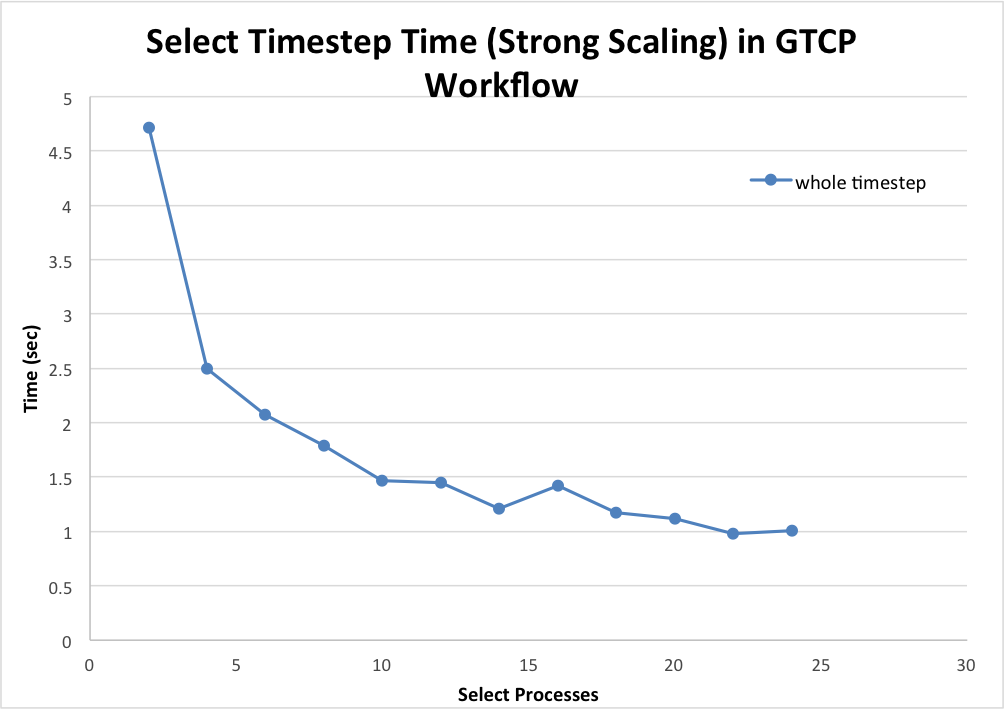
\includegraphics[width=0.3\textwidth]{fig/Titan-GTCP-Strong-Select-1}
\label{fig:gtcp-strong-select-1}
}
\subfigure[Select-2]{
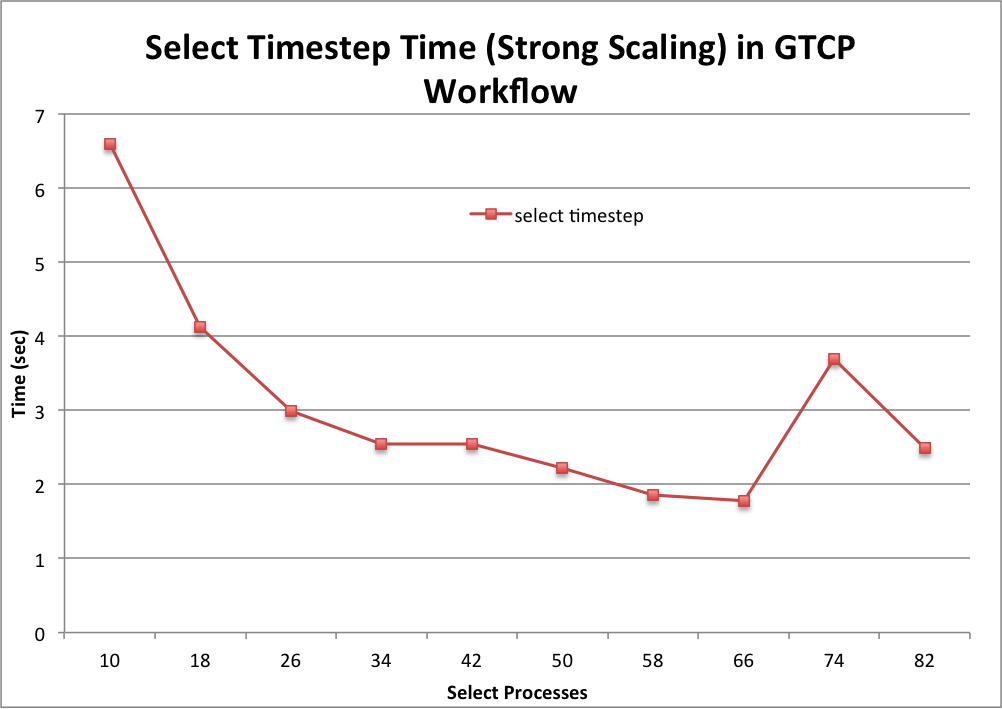
\includegraphics[width=0.3\textwidth]{fig/Titan-GTCP-Strong-Select-2}
\label{fig:gtcp-strong-select-2}
}
\vspace{-0.10in}
\caption{SuperGlue Components Strong Scaling Select For GTCP}
\label{fig:gtcp-strong-select}
\vspace{-0.10in}
\end{figure*}

\begin{figure*}[t!]
\vspace{-0.10in}
\center
\subfigure[Dim-Reduce]{
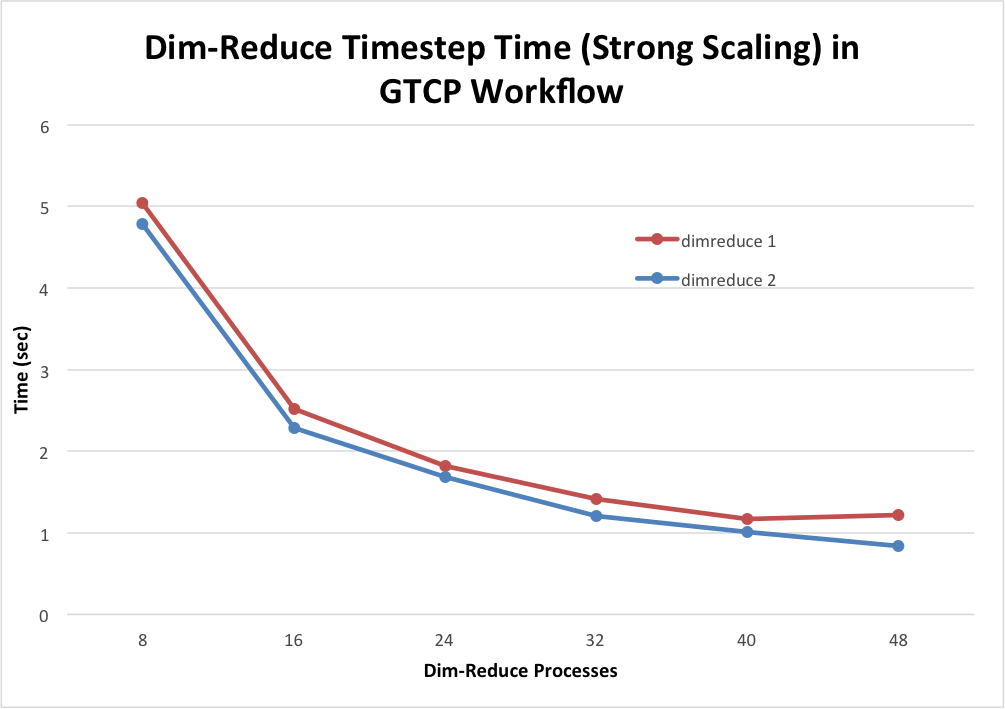
\includegraphics[width=0.3\textwidth]{fig/Titan-GTCP-Strong-Dim-Reduce}
\label{fig:gtcp-strong-dim-reduce}
}
\subfigure[Histogram]{
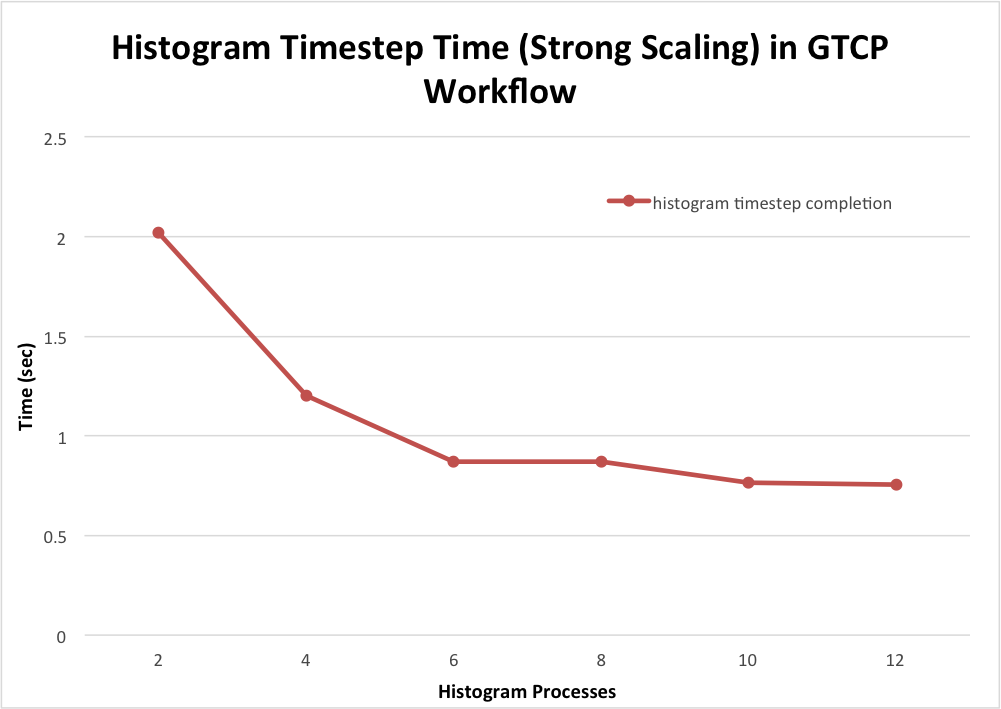
\includegraphics[width=0.3\textwidth]{fig/Titan-GTCP-Strong-Histogram}
\label{fig:gtcp-strong-histogram}
}
\vspace{-0.10in}
\caption{SuperGlue Components Strong Scaling For GTCP}
\label{fig:gtcp-strong}
\vspace{-0.10in}
\end{figure*}

\subsection{Weak Scaling Experiments}

Additional experiments are performed for the GTCP workflow to determine the
weak scaling performance for the components. Additional experiments for the
LAMMPS workflow are not performed since the components are identical and the
data sizes are the only difference. The configurations for these experiments
are presented in Table~\ref{tab:eval-weak-gtcp-1}. The performance results are
presented in Table~\ref{tab:eval-weak-gtcp-2}. To read the tables, match the
rows. For example, the first row in Table~\ref{tab:eval-weak-gtcp-1} corresponds
to the preformance results in row 1 in Table~\ref{tab:eval-weak-gtcp-2}.

{\em Select} gets the full brunt of the total data size. Dividing the process
count into the total data size shows that on average, it is roughly the same
for weak scaling. The other components exhibit similar performance consistency.
Also note that these are not exactly identical ratios or counts.  The data size
per GTCP process is maintained as it is scaled. The amount of data each
SuperGlue component process varies a bit. Also note that there is not a fixed
n-1 ratio required for any of the components. Instead, an m-n mapping works
correctly.

%Process count ratios
%GTCP	GTCP		GTCP
%vs	vs		vs
%Select	Dim-Reduce	Histogram
%6.4	10.67		32
%5.25	8.4		41
%8.67	11.14		34
%9.36	12.31		46.8

\begin{table*}[tbp]
%\vspace{-0.15in}
\centering
\caption{GTCP Weak Scaling Evaluation Configuration Settings}
\label{tab:eval-weak-gtcp-1}
\vspace{-0.15in}
\begin{tabular}{|l|l|l|l|l|l|l|}
\hline
GTCP Procs & Select Procs & Dim-Reduce 1 & Dim-Reduce 2 & Histogram Procs & Total Data Size & End-to-End Time\\
\hline
64 & 10 & 6 & 6 & 2 & 918,303,680 & 92.724\\
\hline
84 & 16 & 10 & 10 & 2 & 1,434,599,936 & 115.232\\
\hline
156 & 18 & 14 & 14 & 4 & 2,065,583,520 & 97.266\\
\hline
234 & 25 & 19 & 19 & 5 & 2,811,256,000 & 96.359\\
\hline
\end{tabular}
\vspace{-0.15in}
\end{table*}

\begin{table}[tbp]
\vspace{-0.10in}
\centering
\caption{GTCP Weak Scaling Component Performance}
\label{tab:eval-weak-gtcp-2}
\vspace{-0.15in}
\begin{tabular}{|p{0.67 in}|p{0.67 in}|p{0.67 in}|p{0.65 in}|}
\hline
Select Average Time & Dim-Reduce 1 Average Time & Dim-Reduce 2 Average Time & Histogram Average Time\\
\hline
1.55 & 1.58 & 1.34 & 0.6\\
\hline
2.34 & 1.58 & 1.72 & 0.78\\
\hline
2.31 & 1.73 & 1.54 & 0.713\\
\hline
2.19 & 1.76 & 1.68 & 0.89\\
\hline
\end{tabular}
\vspace{-0.25in}
\end{table}

\section{Conclusions and Future Work}
\label{s:conclusion}

This paper presents SuperGlue, a demonstration of making generic, reusable
components for scientific simulations. By decomposing the operations into small
chunks, we can achieve components that can be reused, without modification, for
a variety of different workflows. In this work we investigate using a
stream-based structure with generic components to achieve easier to build and
use workflows.  Stream-based, generic workflow components should be designed so
as to allow for the greatest variety in their arrangement and for a maximum
number of downstream subscribers. Designing components with the ability to
handle data having any number of dimensions provides a very useful way to link
them together. Maintaining a high level of semantics upstream, for example by
labeling dimensions and certain quantities inside of these dimensions, gives a
good understanding of the data to downstream components. There is a need for
components that organize the data in a format that downstream components can
understand. And, designing specific disk writer components removes the need to
temporarily modify analytics components to let them also act as disk writers.

Through the demonstration of generating a velocity histogram for LAMMPS, the
molecular dynamics simulation, and a pressure histogram for GTC, the particle
in cell fusion reactor simulator, we achieved reusing the same components in
very different data formats and application types.

While this work leverages ADIOS and the FlexPath transport, this is not the
only approach for addressing reusable components. Other, similar approaches can
also work well. However, in this case, the data annotation provided by this
connection infrastructure help enable reusable components by offering the
necessary metadata to perform the general operations.

There are a number of improvements we can make to our current implementation to
have at our disposal more robust and flexible workflow components. As mentioned
earlier, reading and writing dimension labels at each step in the workflow
provides more information to downstream components and presents a clear
advantage. The ADIOS interface includes the ability to send output to multiple
destinations, by having several ``write groups.'' We wish to explore the
possibility of a {\em Fork Component} that would use this functionality of
ADIOS to allow the creation of branched workflows.

The components we have developed in this research cover only a small portion of
the procedures that computational scientists need in the development of their
workflows. Eventually, we wish to allow for the development of a large
collection of generic workflow components. We can take steps in this direction
by building on our existing components. For example, {\em Magnitude} performs a
relatively simple operation on multi-dimensional data, where one dimension
spans a number of quantities involved in each instance of the operation. This
model can fit any number of operations involving a repeating, fixed number of
quantities, and it can even be made to work with a formula specified by the
user at runtime. This opens the door to a large family of generic components.

Finally, while we have kept performance in mind in the development of these
components, performance optimization is not yet the focus of this research. In
the design of any generic tool however, the question of performance inevitably
arises. Indeed, designing tools that are not meant to operate on a specific
format of input data can easily impact performance. For example, {\em
Dim-Reduce} performs the same amount of computation whether it re-arranges data
or not. In the long run, optimizing these components will involve detecting
such situations where they can avoid performing unnecessary iterations and data
manipulation.

\section*{Acknowledgments}

%
\includegraphics[scale=0.07]{logos/doe_logo}
%
\includegraphics[scale=0.30]{logos/snl_logo}
%
\includegraphics[scale=0.35]{logos/nnsa_logo}
Sandia National Laboratories is a multi-program laboratory managed and operated
by Sandia Corporation, a wholly owned subsidiary of Lockheed Martin
Corporation, for the U.S. Department of Energy's National Nuclear Security
Administration under contract DE-AC04-94AL85000.

This work was supported by Advanced Scientific Computing Research, Office of
Science, U.S. Department of Energy, under Contract DE-AC02-06CH11357, program
manager Lucy Nowell.

\bibliographystyle{abbrv}
\bibliography{gcomps,p,fakeroot,sslab,manycore,conf,whole}

\vfill\eject

\end{document}
